\documentclass{book}

\title{Introduction to Materials Science and Engineering}
\newcommand{\subtitle}{}
\newcommand{\booklicense}{\href{}{Attribution 4.0 International (CC BY 4.0)}}

% authors %
\author{Jonathan Emery \and Kenneth Shull \and Jacob Kelter}
\newcommand{\authoraffiliation}{}

% Create convenient commands \booktitle and \bookauthor
\makeatletter
\newcommand{\booktitle}{\@title}
\newcommand{\bookauthor}{\@author}
\makeatother

% This utf8 declaration is not needed for versions of latex > 2018 but may
% be helpful for older software. Eventually it may not be worth keeping.
%\usepackage[utf8]{inputenc}  

\usepackage{amsmath} % used by equations
\usepackage{siunitx} % used for scientific measurements
\usepackage[version=3]{mhchem} % used for chemical notation
\usepackage{hyperref}
% link options
\hypersetup{
  colorlinks=true,
  linkcolor=purple,
  urlcolor=purple,
  pdftitle={Introduction to Materials Science and Engineering},
  pdflang={en-us},
  pdfcreator={LaTeX via pandoc}
}
\usepackage{booktabs}
\usepackage{longtable}
\usepackage{array}
\usepackage{graphicx}
% sets image width to text body width
\setkeys{Gin}{width=\linewidth,totalheight=\textheight,keepaspectratio}
\usepackage{xcolor}
\definecolor{purple}{HTML}{663399}

% The following dimensions specify 4.75" X 7.5" content on 6 3/8" by 9 1/4"
% paper. The paper width and height can be tweaked as required and the content
% should size to fit within the margins accordingly.
%
% The (inside) bindingoffset should be larger for books with more pages. Some
% standard recommended sizes are .375in minimum up to 1in for 600+ page books.
% Sizes .75in and .875in are also recommended roughly at 150 and 400 pages.
\usepackage[bindingoffset=1in,
            left=1in, 
            right=1in,
            top=1in, 
            bottom=1in,
            paperwidth=8.27in, 
            paperheight=11.69in]{geometry}
% Here is an alternative geometry for reading on letter size paper:
% \usepackage[margin=.75in, paperwidth=8.5in, paperheight=11in]{geometry}

\usepackage[normalem]{ulem} % underlined text

\renewcommand{\contentsname}{Contents} 

% pandoc settings %
\providecommand{\tightlist}{%
  \setlength{\itemsep}{0pt}\setlength{\parskip}{0pt}}

%\newenvironment{Shaded}{
%    \begin{center}
%    \begin{tabular}{|p{0.9\textwidth}|}
%    \hline\\
%    }
%    { 
%    \\\\\hline
%    \end{tabular} 
%    \end{center}
%}

\newenvironment{shaded*}{
    \begin{center}
    \begin{tabular}{|p{0.9\textwidth}|}
    \hline\\
    }
    { 
    \\\\\hline
    \end{tabular} 
    \end{center}
}

\newlength{\cslhangindent}
\setlength{\cslhangindent}{1.5em}
\newlength{\csllabelwidth}
\setlength{\csllabelwidth}{3em}
\newlength{\cslentryspacingunit} % times entry-spacing
\setlength{\cslentryspacingunit}{\parskip}
\newenvironment{CSLReferences}[2] % #1 hanging-ident, #2 entry spacing
 {% don't indent paragraphs
  \setlength{\parindent}{0pt}
  % turn on hanging indent if param 1 is 1
  \ifodd #1
  \let\oldpar\par
  \def\par{\hangindent=\cslhangindent\oldpar}
  \fi
  % set entry spacing
  \setlength{\parskip}{#2\cslentryspacingunit}
 }%
 {}
\usepackage{calc}
\newcommand{\CSLBlock}[1]{#1\hfill\break}
\newcommand{\CSLLeftMargin}[1]{\parbox[t]{\csllabelwidth}{#1}}
\newcommand{\CSLRightInline}[1]{\parbox[t]{\linewidth - \csllabelwidth}{#1}\break}
\newcommand{\CSLIndent}[1]{\hspace{\cslhangindent}#1}

\usepackage{color}
\usepackage{fancyvrb}
\newcommand{\VerbBar}{|}
\newcommand{\VERB}{\Verb[commandchars=\\\{\}]}
\DefineVerbatimEnvironment{Highlighting}{Verbatim}{commandchars=\\\{\}}
% Add ',fontsize=\small' for more characters per line
\newenvironment{Shaded}{}{}
\newcommand{\AlertTok}[1]{\textcolor[rgb]{1.00,0.00,0.00}{\textbf{#1}}}
\newcommand{\AnnotationTok}[1]{\textcolor[rgb]{0.38,0.63,0.69}{\textbf{\textit{#1}}}}
\newcommand{\AttributeTok}[1]{\textcolor[rgb]{0.49,0.56,0.16}{#1}}
\newcommand{\BaseNTok}[1]{\textcolor[rgb]{0.25,0.63,0.44}{#1}}
\newcommand{\BuiltInTok}[1]{#1}
\newcommand{\CharTok}[1]{\textcolor[rgb]{0.25,0.44,0.63}{#1}}
\newcommand{\CommentTok}[1]{\textcolor[rgb]{0.38,0.63,0.69}{\textit{#1}}}
\newcommand{\CommentVarTok}[1]{\textcolor[rgb]{0.38,0.63,0.69}{\textbf{\textit{#1}}}}
\newcommand{\ConstantTok}[1]{\textcolor[rgb]{0.53,0.00,0.00}{#1}}
\newcommand{\ControlFlowTok}[1]{\textcolor[rgb]{0.00,0.44,0.13}{\textbf{#1}}}
\newcommand{\DataTypeTok}[1]{\textcolor[rgb]{0.56,0.13,0.00}{#1}}
\newcommand{\DecValTok}[1]{\textcolor[rgb]{0.25,0.63,0.44}{#1}}
\newcommand{\DocumentationTok}[1]{\textcolor[rgb]{0.73,0.13,0.13}{\textit{#1}}}
\newcommand{\ErrorTok}[1]{\textcolor[rgb]{1.00,0.00,0.00}{\textbf{#1}}}
\newcommand{\ExtensionTok}[1]{#1}
\newcommand{\FloatTok}[1]{\textcolor[rgb]{0.25,0.63,0.44}{#1}}
\newcommand{\FunctionTok}[1]{\textcolor[rgb]{0.02,0.16,0.49}{#1}}
\newcommand{\ImportTok}[1]{#1}
\newcommand{\InformationTok}[1]{\textcolor[rgb]{0.38,0.63,0.69}{\textbf{\textit{#1}}}}
\newcommand{\KeywordTok}[1]{\textcolor[rgb]{0.00,0.44,0.13}{\textbf{#1}}}
\newcommand{\NormalTok}[1]{#1}
\newcommand{\OperatorTok}[1]{\textcolor[rgb]{0.40,0.40,0.40}{#1}}
\newcommand{\OtherTok}[1]{\textcolor[rgb]{0.00,0.44,0.13}{#1}}
\newcommand{\PreprocessorTok}[1]{\textcolor[rgb]{0.74,0.48,0.00}{#1}}
\newcommand{\RegionMarkerTok}[1]{#1}
\newcommand{\SpecialCharTok}[1]{\textcolor[rgb]{0.25,0.44,0.63}{#1}}
\newcommand{\SpecialStringTok}[1]{\textcolor[rgb]{0.73,0.40,0.53}{#1}}
\newcommand{\StringTok}[1]{\textcolor[rgb]{0.25,0.44,0.63}{#1}}
\newcommand{\VariableTok}[1]{\textcolor[rgb]{0.10,0.09,0.49}{#1}}
\newcommand{\VerbatimStringTok}[1]{\textcolor[rgb]{0.25,0.44,0.63}{#1}}
\newcommand{\WarningTok}[1]{\textcolor[rgb]{0.38,0.63,0.69}{\textbf{\textit{#1}}}}

% Content Starts Here
\begin{document}
\frontmatter

% ---- Half Title Page ----
% current geometry will be restored after title page
\newgeometry{top=1.75in,bottom=.5in}
\begin{titlepage}
\begin{flushleft}

% Title
\textbf{\fontsize{48}{54}\selectfont Introduction to Materials Science and
Engineering \\}
\textbf{\large \textit{}}

% Draw a line 4pt high
\par\noindent\rule{\textwidth}{4pt}\\

% authors
\begin{flushright}

      \textbf{Jonathan Emery}, \emph{Northwestern University}\\
      \textbf{Kenneth Shull}, \emph{Northwestern University}\\
      \textbf{Jacob Kelter}, \emph{Northwestern University}\\
  
\end{flushright}

% \vspace{\fill}
\vspace{\fill}

\end{flushleft}
\begin{center}
  %\includegraphics{booksvg.pdf}\\[4pt]
  \fontfamily{lmtt}\small{Northwestern University Libraries\\
  Evanston, IL\\
  https://library.northwestern.edu}
\end{center}
  
\end{titlepage}
\restoregeometry
% ---- End of Half Title Page ----

% Do not show page numbers on colophon page
\thispagestyle{empty}

\begin{flushleft}

\textbf{Copyright \textcopyright{} 2021  The Authors\\
License: \booklicense}\\[11pt] 


For permissions beyond the scope of this license, visit https://library.northwestern.edu

\vspace*{\fill}

\begin{description}
  \item[Recommended Citation] \hfill \\ 
  \item[Publisher] \hfill \\ Northwestern University Libraries, Evanston, IL
  \item[Date] \hfill \\ 2021
    \item[Website] \hfill \\ something
          \item[Subjects] \hfill \\ Academic Libraries, Technology
  \item[keywords] \hfill \\ digital publishing, pandoc, open educational
resources
  
\end{description}


\vspace*{\fill}

This book was typeset using \LaTeX{} software and processed with \href{https://pandoc.org}{Pandoc} using the \href{http://lantern.northwestern.pub}{Lantern} publishing workflow.\\

\end{flushleft}

% A title page resets the page # to 1, but the second title page
% was actually page 3. So add two to page counter.
\addtocounter{page}{2}

% The asterisk excludes chapter from the table of contents.
\chapter*{About this Book}
This text introduces the core topics and foundational concepts of Materials
Science and Engineering. It is structured within the framework of the
Materials Science Paradgm. We cover introductory materials processing,
structure, properties, and performance with particular emphasis on the
relationship between structure and properties. We focus on conventional
materials classes: metals, ceramics, and polymers -aand discuss their various
properties - such as mechanical, electronic, thermal, optical, magnetic, and
electrochemical. Broader themes that arise are how materials' performance
influences technological development, the economy, the environment, and
society. This text is a pilot version intented to leverage computational tools
to assist students in connecting conceptual understanding of materials
science-relevent phenomenon with their mathematical models.

% Three-level Table of Contents
\setcounter{tocdepth}{3}
\tableofcontents

\mainmatter

\hypertarget{preface}{%
\chapter{Preface}\label{preface}}

This text introduces the core topics and foundational concepts of Materials
Science and Engineering. It is structured within the framework of the
Materials Science Paradigm (\textbf{fig:MSEParadigm?}), which focuses in the
causal relationship between materials processing, structural, properties, and
performance (). We cover introductory materials processing, structure,
properties, and performance with particular emphasis on the relationship
between structure and properties. We focus on conventional materials classes:
metals, ceramics, and polymers - and discuss their various properties - such
as mechanical, electronic, thermal, optical, magnetic, and electrochemical.
Broader themes that arise are how materials' performance influences
technological development, the economy, the environment, and society. This
text is a pilot version intended to leverage computational tools to assist
students in connecting conceptual understanding of materials science-relevant
phenomenon with their mathematical models.

\begin{figure}
\hypertarget{fig:MSEParadigm}{%
\centering
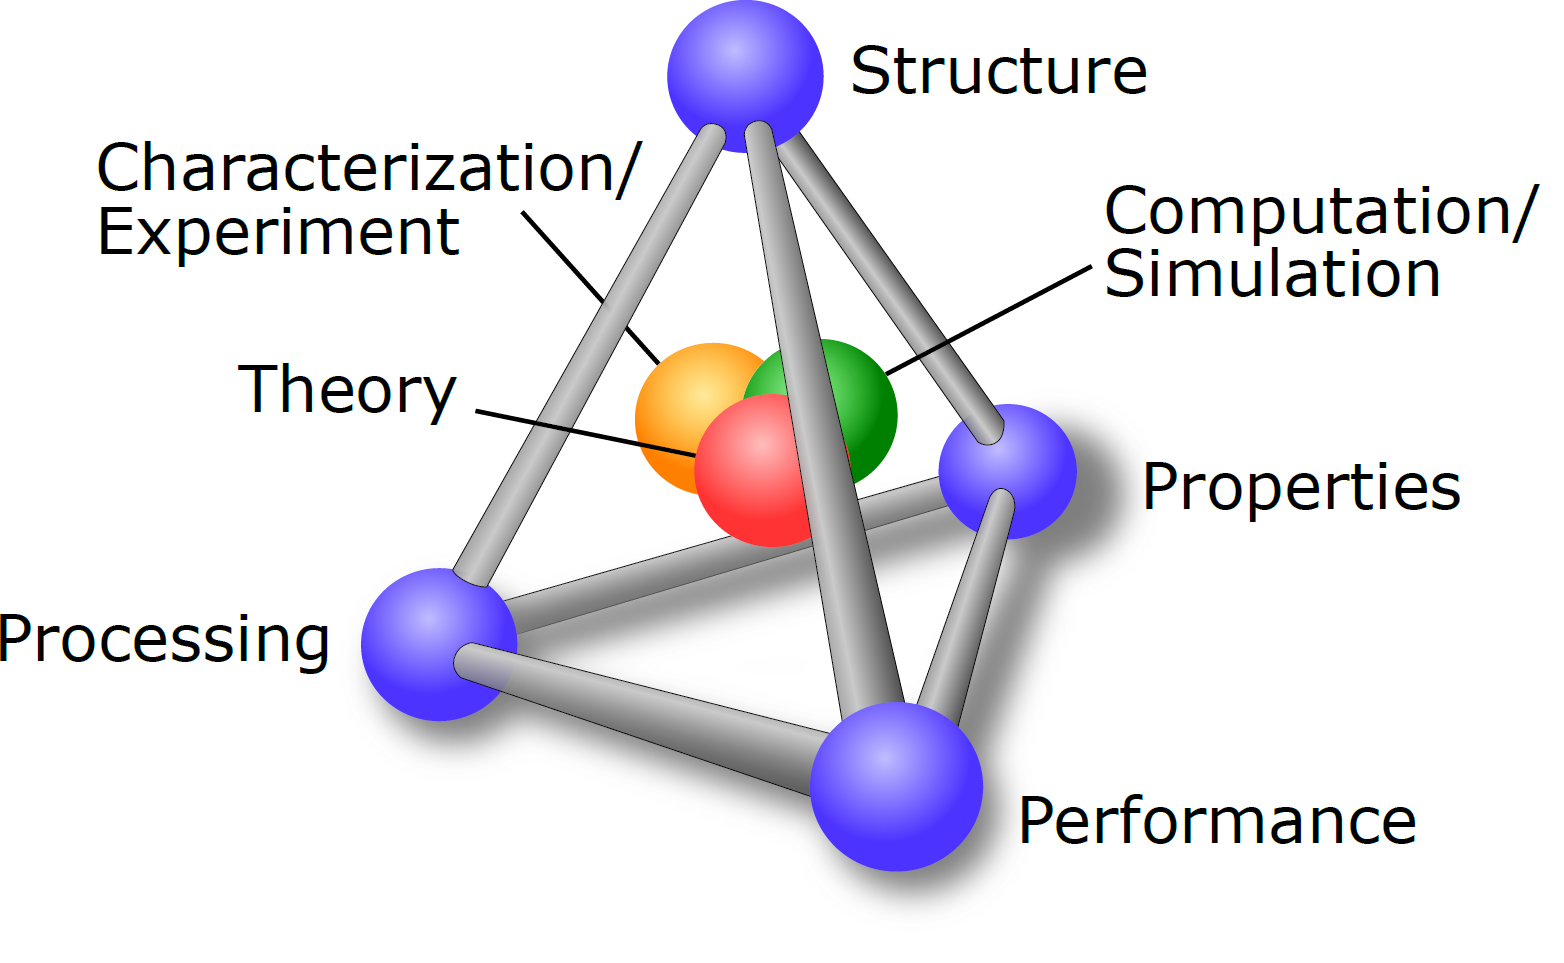
\includegraphics{images/figures/MSE-paradigm.png}
\caption{The Materials Science Paradigm}\label{fig:MSEParadigm}
}
\end{figure}

\hypertarget{bonding-to-crystal-structure}{%
\chapter{Bonding to Crystal Structure}\label{bonding-to-crystal-structure}}

\hypertarget{the-atomic-hypothesis}{%
\section{The Atomic Hypothesis}\label{the-atomic-hypothesis}}

The physicist Richard Feynman opened his famous lectures on physics with the
following question: If, in some cataclysm, all of scientific knowledge were to
be destroyed, and only one sentence passed on to the next generation of
creatures, what statement would contain the most information in the fewest
words?

It's certainly an interesting question, and here is Feynman's own answer:

\begin{quote}
I believe it is the atomic hypothesis that all things are made of atoms ---
\emph{little particles that move around in perpetual motion, attracting each
other when they are a little distance apart, but repelling upon being squeezed
into one another}. In that one sentence, you will see, there is an enormous
amount of information about the world, if just a little imagination and
thinking are applied.
\end{quote}

There is indeed an enormous amount of information in that one sentence, but
let's see if we can make it even shorter. What if we just said ``All things
are made of atoms --- tiny entities that move around in perpetual motion.''?
Could we deduce from this short sentence that they attract each other when
they are a little distance apart, but repel when squeezed into one another?
From simple observations of the world around us, we can. If atoms never
attracted one another, then solids and liquids would never form. On the other
hand, if atoms didn't repel one another when squeezed close enough together,
then matter would collapse into a single point. (LeSar 2013)

So, we've kept the essential information and reduced the number of words to
14. Not bad! However, our statement is entirely \emph{qualitative}. It won't
let us make any predictions beyond what we've already stated: that solids and
liquids will form but matter won't collapse. In the coming sections we will
construct a foundational \emph{quantitative} model of the atomic hypothesis
and see if it is useful. That is, what can we \emph{explain} with this model,
and what can we \emph{predict} with it? But first, we will briefly address why
Feynman calls his statement the atomic ``hypothesis'' as opposed to ``theory''
or ``fact'' and how we will use models to understand materials.

\hypertarget{scientific-hypotheses-theories-and-models}{%
\section{Scientific Hypotheses, Theories, and
Models}\label{scientific-hypotheses-theories-and-models}}

When Feynman gave his lectures in 1963, the existence of atoms was scientific
fact. Indeed, already by 1908, the biggest skeptics of the atomic hypothesis
had finally been persuaded by the evidence (Crawford 1984). So, why did
Feynman call it the atomic ``hypothesis'' a half a century after it was
established as fact? He doesn't say explicitly, but one possibility is that he
was describing a thought experiment in which we only can pass only a single
sentence of scientific knowledge to the next generation. For that generation,
the statement would indeed be a \emph{hypothesis}, as they would not yet have
any evidence for it. Based on other parts of the lecture, Feynman also wanted
to discuss his view of how science works: in short, we use imagination
combined with evidence to construct physical laws that help us understand the
universe. We then perform experiments to test these laws. At the end of the
lecture Feynman says: ``How do we know that there are atoms? By one of the
tricks mentioned earlier: we make the \emph{hypothesis} that there are atoms,
and one after the other results come out the way we predict, as they ought to
if things are made of atoms.''

Already in Feynman's time, and certainly today, we can rightfully talk about
the atomic ``theory'' instead of ``hypothesis.'' In everyday language, people
use the word ``theory'' to mean something more like ``hypothesis'' (e.g.~my
theory of why that happened is\ldots). The word ``theory,'' in physical
science is properly used to refer to a set of ideas about how the universe
works that have been thoroughly tested and are widely accepted as fact. Of
course, scientists are people too and sometimes use the word ``theory'' in the
more colloquial sense, which is pretty confusing.

But what is a scientific theory exactly? The words ``theory'' and ``theater''
share the same Greek root ``thea'' which means ``a view.'' You can think of a
theory as a way of conceptually ``viewing'' nature that allows you to ``see''
it in a new and powerful way. What truly separates a scientific theory from an
everyday theory, however, is that the concepts of a scientific theory are
linked with precise mathematical and/or computational representations which
are further related to measurements we can take in the real world. This is
true of a well-formed scientific hypothesis as well. What separates a
scientific hypothesis from a theory is, basically, how much evidence supports
it.

We will refer to mathematical and computational representations of specific
phenomena as ``models.'' We build models at every stage of the scientific
process. A model can be a hypothesis of how things work. It can also be the
application of a widely accepted theory to understand a specific situation. A
model is similar to a map. A geographical map represents where things are in
relation to one another. The world ``presents'' the actual geography and the
map represents it. (That is, \emph{re}presents it in a new way.) The map is
not the same thing as the territory it represents, and in order to be useful,
the map has to simplify. If it were just as detailed as the real world, it
would be just as hard to understand. \textbf{All models}, not just maps, are
\textbf{approximations/simplifications of reality}. The statistician George
Box put it this way:

\begin{quote}
Now it would be very remarkable if any system existing in the real world could
be exactly represented by any simple model. However, cunningly chosen
parsimonious models often do provide remarkably useful approximations. For
example, the law \(PV = RT\) relating pressure \(P\), volume \(V\) and
temperature \(T\) of an ``ideal'' gas via a constant \(R\) is not exactly true
for any real gas, but it frequently provides a useful approximation and
furthermore its structure is informative since it springs from a physical view
of the behavior of gas molecules. For such a model there is no need to ask the
question ``Is the model true?''. If ``truth'' is to be the ``whole truth'' the
answer must be ``No''. The only question of interest is ``Is the model
illuminating and useful?'' (Box 1979)
\end{quote}

Understanding this, we might provide a slightly more nuanced answer to the
question ``How do we know that there are atoms?: We have constructed models of
atoms and their predictions match experiments! However, except for the
simplest of cases (e.g.~a single hydrogen atom), and using our most
sophisticated models (e.g.~quantum mechanics),''matching experiments'' means
only approximately matching.

In our study of materials science and engineering, we will use many types of
models including both mathematical and computational models. None of them will
represent the ``whole truth'' about materials, but they will each be
illuminating and useful for something. Let's get started with our first one.

\hypertarget{modeling-the-atomic-hypothesis-with-interatomic-potentials}{%
\section{Modeling the Atomic Hypothesis with Interatomic
Potentials}\label{modeling-the-atomic-hypothesis-with-interatomic-potentials}}

When building a model, you first have to decide what the entities of your
model will be. In this course, we will typically model atoms as Newtonian
objects (i.e.~point objects with position and velocity) that exert forces on
each other. While this is clearly ``wrong'', as atoms (and therefore many of
their properties) are quantum mechanical in nature, we won't worry too much
about that at this point. As we move forward, we encourage that you keep mind
concepts regarding atomic structure as covered in the Chemistry Review
session.

Instead of spending to much time on atomic orbitals and electron
configurations, we'll start with a review of the physical definitions of force
and potential energy and then use those concepts to construct our model.

\hypertarget{review-of-force-and-potential-energy}{%
\subsection{Review of Force and Potential
Energy}\label{review-of-force-and-potential-energy}}

Let's consider an idealized spring, shown in (\textbf{fig:SpringSystem?}),
which is governed by Hooke's Law. This spring is oriented in the
\(x\)-direction, and one end is positioned at \(x = 0\) when in equilibrium.
When displaced in the positive \(x\)-direction, there is a restoring force
\(F\) acting to pull the spring's end back to \(x=0\) that is linearly
proportional to the distance the end of the spring was displaced, \(x\).
Similarly, when compressed along the \(-x\)-direction, there is a restorative
force acting the the \(+x\) direction. Hooke's Law is written as

\begin{equation}   F(x) = -k x \end{equation}\{\#eq:hooke\}

where \(k\) is the spring constant - a measure of how stiff the spring is. A
higher \(k\) means a larger restoring force when the spring is displaced.
(\textbf{fig:SpringSystem?}) displays a red (solid) line that follows Hooke's
law (\textbf{eq:hooke?}) as a function of \(x\).

\begin{figure}
\hypertarget{fig:SpringSystem}{%
\centering
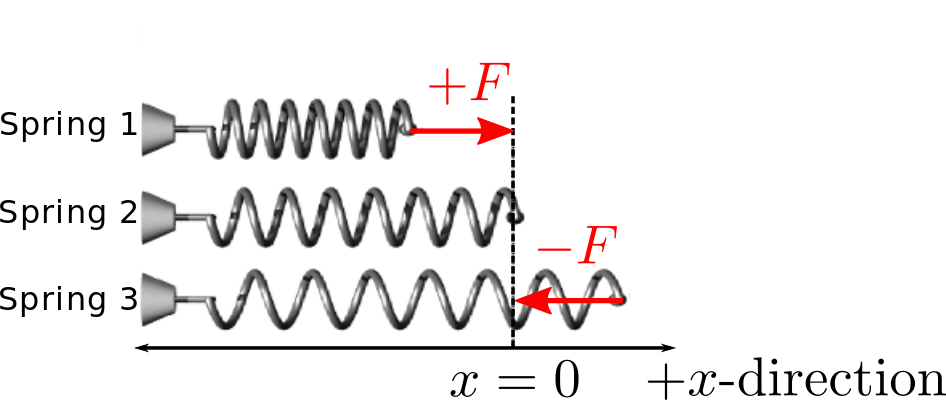
\includegraphics{images/figures/SpringSystem.png}
\caption{Three springs with equilibrium (\(F=0\)) positions of \(x=0\). Spring
1 is in compression, with restorative force acting in the \(+x\) direction.
Spring 2 is at equilibrium. Spring 3 is in tension, with restorative force
acting in the \(-x\) direction.}\label{fig:SpringSystem}
}
\end{figure}

We relate the force and the potential energy \(U(x)\) as a function of \(x\)
by

\begin{equation}  F(x) = - \frac{dU(x)}{dx} \end{equation}\{\#eq:pe\}

Below, the \(U(x)\) is plotted as the purple dashed line. (\textbf{eq:pe?})
says that the restoring force is equal the the derivative of the potential
energy function. Intuitively, you can think of the potential function as a
landscape that a ball is rolling around in. The ball feels force that causes
it to roll downhill. The magnitude of that force is proportional to the slope
at the the position it is located. When potential energy is at a local minimum
the force is zero (it is at equilibrium). The further the ball is displaced
from this local minimum, the higher its energy.

\hypertarget{concept-check-questions}{%
\subsubsection{Concept Check Questions}\label{concept-check-questions}}

Take a few minutes to answer the following questions before you continue.

\textbf{Q1.1: Based on Hooke's Law and the equation for potential energy, why
is the general shape of energy curve parabolic? Do some math to show us why.}

Potential energy is defined as \(dU/dx = -F(x)\), so we can plug in the
expression for \(F(x) = -kx\) and integrate:

\begin{align*}   U(x) &= \int kx\,dx\\    U(x) &= \frac{1}{2}kx^2 + C \end{align*}

This is a parabolic equation. The constant \(C\) determines our reference
point. If, for example (and this is a fine idea, here) we decide that we want
\(U(x=0 \,\text{m}) = 0 \,\text{N-m}\), then \(C = 0 \,\text{N-m}\).

Let's make sense of this intuitively.

\begin{enumerate}
\def\labelenumi{\arabic{enumi}.}
\tightlist
\item
  The potential energy stored in the spring is a function of how far it is
  from equilibrium. The further it is from equilibrium, the higher the
  potential energy.
\item
  In order to stretch/compress the spring, you have to exert a force on it
  which increases linearly with displacement. As you stretch the spring, the
  larger the restorative force (the harder it is to pull): \(F(x)=-kx\).
\item
  Now let's relate steps 1. and 2. The potential energy of the spring depends
  on how far it is stretched, and stretching it gets harder and harder the
  larger the displacement. So, for any little distance, \(dx\), that the
  spring is stretched the potential energy should increase more than it did
  for the previous little distance, \(dx\). This explains intuitively why the
  potential energy is super-linear, but to get the exact parabolic shape, you
  need to do the math.
\item
  Mathematically, the potential energy is the sum of the force \(F(x)\)
  exerted on the spring times the displacement that force was exerted through,
  \(dx\), i.e.~the integral of the force function \(F(x)\) over the
  displacement: \(U(x)= -\int F(x)dx\). The negative sign in this equation
  exists because the we've defined our force as a restorative force. This
  convention makes the energy increase as the displacement increases in
  \emph{either} the \(-x\)- or \(+x\)-directions.
\end{enumerate}

\textbf{Q1.2: Assume that the spring constant \(k = 1\,\mathrm{N/m}\), What is
the potential energy of the spring when stretched to \(1 \,\mathrm{m}\)? How
about \(2 \,\mathrm{m}\)?{}``}

To find the equation for the potential energy of the spring, we integrate from
equilibrium \(x=0\) to the displaced value \(x_f\) (we've dropped units below
for simplicity):

\begin{align*}   U(x) &= k\int_0^{x_f} x\,dx\\   U(x) &= \frac{1}{2}kx_f^2 \end{align*}

So:

\begin{align*}   U(1\,\text{m}) &= 0.5\text{N-m}\\   U(2\,\text{m}) &= 2\text{N-m} \end{align*}

You can confirm this on the graph by setting \(k=1\,\text{N-m}\) and finding
the value of \(U\) at the values of \(x\).

\textbf{Q1.3: What happens to the force and the potential energy curves when
the spring constant is increased? Describe in words after playing with the
model.}

As the spring constant increase, the slope of the force function increases
along the entire domain. This makes sense, the spring becomes stiffer the
spring constant increases, and so the restorative force increases as \(k\)
increase.

Similarly, the potential energy function (the parabola) appears to
``contract'' towards the origin as \(k\) increases. This makes sense, a stiff
spring will possess more energy at some value of \(x\) compared to a less
stiff (more compliant) spring. That is, it takes more energy to displace the
spring over each \(dx\).

\hypertarget{sketching-a-potential-energy-function-for-interatomic-interactions}{%
\subsection{Sketching A Potential Energy Function for Interatomic
Interactions}\label{sketching-a-potential-energy-function-for-interatomic-interactions}}

In this section we'll introduce a \emph{NetLogo} molecular dynamics model of
two atoms interacting with each other. \emph{NetLogo} is a programming
language designed specifically for to model the interaction and behaviors of
multiple entities, or ``agents''. In materials science, these are often atoms
or molecules. A molecular dynamics model treats molecules and atoms as
Newtonian objects with position, velocity and mass. They accelerate due to
forces they exert on one another (and sometimes external forces) and move
according to Newton's laws. The potential energy that results from the
interaction of the atoms, and therefore the force the atoms feel from each
other, is modeled using a function called an \emph{interatomic potential}.
These interatomic potentials come in lots of different varieties - we'll first
explore how these potentials work in a computational model that we provide,
and then we'll later show you some mathematical models that we can manipulate
to derive important metrics such as equilibrium bond energies and distances.

In this
\href{https://ct-stem.s3.amazonaws.com/uploads/jzkelter/2021/08/18/draw\%20potentials_2021-08-18-19-15-15-372549.html?speed=0.8}{\emph{NetLogo}
model}, you will draw the interatomic potential function and see how the atoms
react. The video demo embedded below shows how to use the model and
demonstrates how you can draw an interatomic potential function similar to the
potential energy function for an ideal spring that you reviewed above. For
simplicity, the left atom is held fixed and only the right atom moves. You can
think of this as looking at the word from the perspective (reference frame) of
the left atom. From an outside perspective, both atoms would be moving. The
force the right atom feels will be proportional to the slope of the
interatomic potential function at its current location.

Your job is to draw an interatomic potential function to model the way you
think atoms behave, using the \protect\hyperlink{SketchModel}{embedded model}.
We have already stated in the atomic hypothesis that atoms repel each other
when squeezed together and attract each other when they are further apart. We
can also deduce from observation that atoms must not attract each other very
much when they are \emph{very} far apart, because otherwise everything would
quickly condense into one giant blob.

\hypertarget{concept-check-questions-1}{%
\subsubsection{Concept Check Questions:}\label{concept-check-questions-1}}

Now we'll spend a few minutes exploring the construction of models that will
align with the atomic hypothesis. Answer the questions below. In the next
section we will introduce a formal mathematical model of the interatomic
potential function based on what we observe here.

\textbf{Q1.4: First, construct a spring potential like that in the model
below. Make some observations about how the atom behaves at different
positions. Which features does the spring model have that fits atomic
hypothesis? What is it missing?}

Here are some general observations for the idealized spring:

\begin{enumerate}
\def\labelenumi{\arabic{enumi}.}
\tightlist
\item
  If the particle is at equilibrium, it stays put. If we stretch it, it will
  move back towards equilibrium.
\item
  The larger the displacement, the larger the restorative force, and the
  quicker it accelerates.
\item
  The atom will oscillate back and forth around equilibrium with large
  amplitude depending on how much energy we give it initially.
\end{enumerate}

The spring potential has a few features that mesh well with our atomic
hypothesis:

\begin{enumerate}
\def\labelenumi{\arabic{enumi}.}
\tightlist
\item
  At some little distance they attract each other.
\item
  When put too close together, they repel.
\item
  They move around in perpetual motion (when they have a bit of energy, at
  least).
\end{enumerate}

However, Feynman implies in \protect\hyperlink{the-atomic-hypothesis}{his
hypothosis} that at large distances, there's really no interaction. We mention
this above as well - if the attraction was large at large distances, all
matter would collapse to a giant blob! The spring potential models
\emph{increasing} forces of attraction at very large distances, which is not
physical and not consistent with the atomic hypothesis.

\textbf{Q1.5: Now, construct an interatomic potential that more accurately
models the atomic hypothesis. What is the main difference between your new
potential and the spring potential? Make some observations about the behavior
of the atomic pair in this potential.}

The main difference in this potential and the spring potential is that we
gradually reduce the force of attraction (by flattening the interatomic energy
curve) as we move further away from equilibrium. We set the potential to
\emph{zero} as the interatomic distance \(x \rightarrow \infty\) This causes
the following effects:

\begin{enumerate}
\def\labelenumi{\arabic{enumi}.}
\tightlist
\item
  When the atoms are close together, the interaction is very similar to the
  spring potential, there is a strong, repulsive force that pushes the atoms
  away from each other.
\item
  There is still a value at which the energy is minimized and the force is
  zero. This is equilibrium.
\item
  When the atoms are placed at larger \(x\), the interaction is very weak and
  they approach each other more slowly. This is good, because we expect their
  interaction to diminish at large distances.
\item
  At very large distances, there is essentially no force
  (\(\frac{dU(x)}{dx} = -F \approx 0\)), and therefore no acceleration. This
  is good! Now atoms that are far enough away essentially ignore each other!
\end{enumerate}

\hypertarget{the-lennard-jones-potential}{%
\subsection{The Lennard-Jones Potential}\label{the-lennard-jones-potential}}

Now that you have worked to figure out what sort of shape an interatomic
potential must have, we will look at one of the simplest mathematical
functions used to model interatomic potentials. (Note, there are
\href{https://www.ctcms.nist.gov/potentials/}{hundreds} of these potentials
that serve to model all sorts of phenomena - not just materials. These
potentials are used by chemists, physicists, biologists, and engineers to
better understand and predict all sorts of physical behavior!)

The Lennard-Jones (LJ) potential, named after Sir John Edward Lennard-Jones,
specifies the potential energy between two atoms, \(U_{\text{LJ}}\), as
function of the distance between them, \(r\) (generalized from \(x\)):

\[
U_{\text{LJ}} = 4 \epsilon \left[\Big(\frac{\sigma}{r}\Big)^{12}-\Big(\frac{\sigma}{r}\Big)^6\right]
\]\{\#eq:LJ\}

The two positive constants, \(\sigma\) and \(\epsilon\), can be adjusted to
model different behaviors and yield different depths and widths to the
potential. These constants are not derived. hey are parameters of the model
that can be adjusted to fit experimental data. What they represent will be
discussed below. Where do the exponents 12 and 6 come from? The 6th power term
can be derived from quantum mechanical considerations due to the effect of
fluctuating electron clouds. Interestingly, the 12th power term cannot
actually be derived from more fundamental theory. It was selected for
mathematical convenience and efficiency, but it serves well to model the
interaction between atoms (and molecules) from the quantum mechanical
phenomenon of Pauli repulsion.

The figure below shows \protect\hyperlink{LJPotential}{an interactive graph of
the LJ potential} along with each of the terms graphed separately. We, we plot
\(+\Big(\frac{\sigma}{r}\Big)^6\) (not \(-\Big(\frac{\sigma}{r}\Big)^6\)) so
you can better see which term is larger as well as when the cross-over of the
two terms occurs. Use the graph to answer a few questions about the potential,
below (which are also reproduced in your homework). We suggest you spend a bit
of time wrestling with the question either yourself or with a partner.
Engaging with the questions in this way will allow you to explore the model
more deeply and help to improve your understanding. These questions aren't
meant to bog you down, however. If you feel stuck after a few minutes, we
recommend looking at the answer (toggle the solution button or look at the
posted solutions on \emph{Perusall}) to make sure you understand it.

\textbf{Q1.6: Which of the terms in the LJ potential (Eq. (\textbf{eq:LJ?}))
is an ``attractive'' term? Which is repulsive?{}``\}}

The \(-\Big(\frac{\sigma}{r}\Big)^6\) term models attraction (note that it is
always negative for positive values of \(r\). \(\sigma\) is always positive).
The \(\Big(\frac{\sigma}{r}\Big)^{12}\) models repulsion and is always
positive.

\textbf{Q1.7: What happens to the interatomic potential energy as the distance
between the atoms gets very large (\(r \rightarrow \infty\))? Show this
mathematically. What does this value at \(U(r \rightarrow \infty)\) mean?}

As \(r \rightarrow \infty\), \(U \rightarrow 0\). This is because both LJ
terms have \(r\) in the denominator, so both go to zero at large values of
\(r\):

\begin{align*}   U_{\text{LJ}}(r \rightarrow \infty) &= 4 \epsilon \left[\Big(\frac{\sigma}{\infty}\Big)^{12}-\Big(\frac{\sigma}{\infty}\Big)^6\right]\\    U_{\text{LJ}}(r \rightarrow \infty) &= 0 \end{align*}

This value of \(U = 0\) is simply convention - atoms that are very far apart
would logically have an energy of zero because they aren't interacting in any
significant way. A good place to set energy to zero.

\textbf{What happens to the interatomic potential energy as the distance
between the atoms gets very small (\(r \rightarrow 0\))? What does this mean?}

Here, we need to compare the magnitude of the attractive \(U_{\text{A}}\) and
repulsive (\(U_{\text{R}}\)) terms as \(r \rightarrow 0\). As \(r\) gets very
small, the term with the larger exponent will dominate, approaching infinity
much faster than term with the smaller exponent, in this case, that's the
repulsive term \(U_{\text{R}} = \Big(\frac{\sigma}{r}\Big)^{12}\). If you'd
like to check, you can also take the ratios of limit and find that:

\begin{equation}   \lim_{r\rightarrow0} \frac{U_{\text{R}}(r)}{U_{\text{A}}(r)} = -\infty \end{equation}

meaning that the repulsive term dominates. This means that atoms that are very
close together are in an extremely unfavorable configuration and will repel
each other strongly. This make sense - two atoms cannot occupy the same
location!

\textbf{Q1.9: The LJ potential (and indeed other interatomic potentials) are
constructed such that the potential energy is positive at short distances,
goes negative as \(r\) increases, reaches a minimum, and then increase and
approach zero at \(r \rightarrow \infty\). What does the negative potential
energy minimum represent?}

This represents the energy needed to break the bond. The system will tend
towards the lowest energy state (the potential energy minimum) and form a
``bond''. To break this bond you need to put energy into the system to somehow
pull the atoms apart. So, if the bond energy is (e.g., for a pair of ions like
Na and Cl) \(U_{\text{0}} =\) 4.26 eV, the well will have a depth of -4.26 eV.
You need to put in 4.26 eV to dissociate the Na and Cl bond. This is
effectively pulling the atoms to \(r \rightarrow \infty\).

\textbf{Find the general expression for the distance at which the potential
energy is minimized. We call this the equilibrium bond distance \(r_0\), and
it is the point of at which net force in the system is zero. Hint: how are
potential energy and force related, and how would you manipulate Eq.
(\textbf{eq:LJ?})) to find this \(r_0\)?}

We want to find the value \(r\) at which \(F = 0\). We can find the net force
in the system by taking the derivative of the potential energy
((\textbf{eq:pe?})):

\begin{equation*}   \frac{dU}{dr} = -F = -\left[-12\Big(\frac{\sigma^{12}}{r^{13}}\Big)+6\Big(\frac{\sigma^6}{r^7}\Big)\right] \end{equation*}

Now, since we are interested at the point of equilibrium, we set this
expression such that the force \(F\) is zero and simplify.

\begin{align*}   F = 0 &= \left[12\Big(\frac{\sigma^{12}}{r_0^{13}}\Big)-6\Big(\frac{\sigma^6}{r_0^7}\Big)\right]\\   12\Big(\frac{\sigma^{12}}{r_0^{13}}\Big)&=6\Big(\frac{\sigma^6}{r_0^7}\Big)\\   r_0 &= 2^{1/6}\sigma \end{align*}

So, if we have some value for \(\sigma\), we can derive the interatomic bond
distance.

\textbf{Q1.11: What happens when you change \(\sigma\)? What do you think we
might be able to model by changing \(\sigma\)?}

What happens when you change \(\epsilon\)? What do you think we might be able
to model by changing \(\epsilon\)?{}``\}

The equilibrium distance between the atoms changes. Increasing \(\sigma\)
would allow us to model larger atomic pairs. Smaller \(\sigma\)s would model
smaller atomic pairs. Increasing \(\sigma\) also \emph{broadens} the well
itself, modeling a more compliant (stretchy) bond.

The depth of the well changes when we change \(\epsilon\). You would adjust
this parameter to model different bond strengths.

\hypertarget{lj-potential-summary}{%
\subsubsection{LJ-potential Summary}\label{lj-potential-summary}}

Now that you have spent some time exploring the LJ-potential, let's summarize.

\begin{itemize}
\tightlist
\item
  The negative 6th-term models the attraction of atoms.
\item
  The positive 12th-term models the repulsion of atoms.
\item
  Both potential energy terms approach zero as \(r \rightarrow \infty\). The
  12th-term goes to zero faster as \(r \rightarrow \infty\) which gives the
  potential its attractive ``tail''.
\item
  Both potential energy terms approach infinity as \(r \rightarrow 0\). The
  12th-term goes to infinity faster as \(r \rightarrow 0\) which dominates the
  energy at small values of \(r\).
\item
  At intermediate distances (typically on the order of a few Å in most
  systems), the attractive and repulsive terms cancel out, achieving
  equilibrium (a minimum where \(F = 0\)) at \(r_0\).
\item
  At values larger than \(r_0\), the atoms are attracted (although very weakly
  as \(r\) increases).
\item
  At values smaller than \(r_0\), the atoms are repelled.
\end{itemize}

In all, we have an interatomic potential function for which atoms repel each
other when squeezed very close together, attract each other at moderate
distances and essentially do not interact at large distances.

In the next section we will use the LJ-potential into a molecular dynamics
simulation with more than two atoms and observe some properties of materials
that can be explained by the interatomic potential model.

\hypertarget{emergent-properties-from-the-lennard-jones-potential}{%
\subsection{Emergent Properties from the Lennard-Jones
Potential}\label{emergent-properties-from-the-lennard-jones-potential}}

The \emph{NetLogo} model below is similar to the one you used earlier, but
now, instead of you drawing the interatomic potential, it is modeled by the
Lennard-Jones potential. You will see the two atoms with the LJ potential
drawn between them from the perspective of the red atom.

Again, in reality, both atoms would feel a force from the interatomic
potential and both would move, but for simplicity, we are holding the green
atom fixed and just attending to the red atom. The red atom starts at \(r_0\),
the distance which minimizes the potential energy. Use the model to answer the
questions below through which you will observe several properties of
materials.

\hypertarget{evaluating-the-lennard-jones-potential}{%
\subsection{Evaluating the Lennard-Jones
Potential}\label{evaluating-the-lennard-jones-potential}}

The LJ potential is a useful model, but like all models, it has limitations.
To evaluate a model, we have to evaluate it in light of the purpose(s) it is
meant to serve. Often people think that scientific models are only meant to
predict, but models can serve other purposes. A model can explain a phenomenon
without making precise predictions. For example, the model of plate tectonics
explains why earthquakes happen, but we still can't predict exactly when they
will happen (we can, however, predict the general areas they will happen based
on the locations of tectonic plates). Other reasons for constructing models
include helping us reason about phenomena, honing our intuitions, and helping
us design technologies. Sometimes there are trade-offs between different
purposes of models. Most prominently, the models that are best at prediction
are often the hardest to understand, making them less useful for helping us
hone our intuitions and reason about a phenomenon.

In reflecting on the model we built we can ask ourselves a couple questions:

\begin{itemize}
\item
  How is this model useful? It hold values because it:

  \begin{itemize}
  \tightlist
  \item
    Allows us to better conceptualize interatomic interactions.
  \item
    Predicts real phenomenon such as thermal expansion, melting temperature,
    and simple crystalline packing structures, and dependence of melting
    temperature vs number of atoms in the system.
  \end{itemize}
\item
  How is this model limited?

  \begin{itemize}
  \tightlist
  \item
    \textbf{Imprecise predictions} The LJ-potential is simple in form, but
    doesn't capture the precise details of real interactions between atoms,
    which are founded in quantum mechanics. Scientists and engineers have made
    some simple adjustments to improve the quantitative predictive ability of
    the LJ-potential, of course, which better match physical observation.
  \item
    \textbf{Unaccounted-for phenomenon} Speaking of quantum mechanics, an
    obvious limitation of the LJ potential is that it cannot model any quantum
    phenomenon.
  \end{itemize}

  The LJ potential is also ignorant of the existence of electron. This means
  it can tell us nothing about the (e.g.) electrical or optical properties of
  materials, as they depend on the behavior of electrons and their
  interactions with photons. The LJ potential is largely limited to physical
  and mechanical behaviors of materials.

  \begin{itemize}
  \tightlist
  \item
    \textbf{Directional Bonding} The LJ potential can only model bonds that
    are non-directional, because the LJ potential only depends on the absolute
    distance between atoms, not their relatively orientations. Non-direction
    bonding does occur in many materials and results in close-packed
    structures (e.g., solid phases of group 18 elements (He, Ne, Ar\ldots)).
    However, there are many different crystal structures that form due in part
    to the influence of bond directionality. The LJ potential will not be able
    to predict these structures.
  \end{itemize}
\end{itemize}

In summary, makes it easy to understand and therefore useful for qualitatively
explaining and reasoning about various mechanical properties of materials. For
this reason, we will continue to use it at various points in the course.
However, the simplicity of the LJ-potential means that there are many
phenomena it can't explain. For those phenomena, we will need other models.

\hypertarget{siunitx-package}{%
\chapter{siunitx Package}\label{siunitx-package}}

\hypertarget{tex-code}{%
\section{TeX Code}\label{tex-code}}

\begin{Shaded}
\begin{Highlighting}[]
\NormalTok{ n(O2)\&=}\FunctionTok{\textbackslash{}SI}\NormalTok{\{.15\}\{}\FunctionTok{\textbackslash{}mol}\NormalTok{\}}\FunctionTok{\textbackslash{}qquad\textbackslash{}qquad}\NormalTok{ \&n(Fe3O4)\&=}\FunctionTok{\textbackslash{}SI}\NormalTok{\{0.3\}\{}\FunctionTok{\textbackslash{}mol}\NormalTok{\}}
\end{Highlighting}
\end{Shaded}

\hypertarget{rendering}{%
\subsection{Rendering}\label{rendering}}

{[} n(O2)\&=\SI{.15}{\mol}\qquad\qquad\&n(Fe3O4)\&=\SI{0.3}{\mol} {]}

\hypertarget{tex-code-1}{%
\section{TeX Code}\label{tex-code-1}}

\begin{Shaded}
\begin{Highlighting}[]
  \FunctionTok{\textbackslash{}si}\NormalTok{\{kg.m.s\^{}\{{-}1\}\}                }\FunctionTok{\textbackslash{}\textbackslash{}}
  \FunctionTok{\textbackslash{}si}\NormalTok{\{}\FunctionTok{\textbackslash{}kilogram\textbackslash{}metre\textbackslash{}per\textbackslash{}second}\NormalTok{\} }\FunctionTok{\textbackslash{}\textbackslash{}}
  \FunctionTok{\textbackslash{}si}\NormalTok{[per{-}mode=symbol]}
\NormalTok{    \{}\FunctionTok{\textbackslash{}kilogram\textbackslash{}metre\textbackslash{}per\textbackslash{}second}\NormalTok{\}  }\FunctionTok{\textbackslash{}\textbackslash{}}
  \FunctionTok{\textbackslash{}si}\NormalTok{[per{-}mode=symbol]}
\NormalTok{    \{}\FunctionTok{\textbackslash{}kilogram\textbackslash{}metre\textbackslash{}per\textbackslash{}ampere\textbackslash{}per\textbackslash{}second}\NormalTok{\}}
\end{Highlighting}
\end{Shaded}

\hypertarget{rendering-1}{%
\subsection{Rendering}\label{rendering-1}}

{[} \si{kg.m.s^{-1}} \textbackslash{} \si{\kilogram\metre\per\second}
\textbackslash{} \si[per-mode=symbol]     {\kilogram\metre\per\second}
\textbackslash{}
\si[per-mode=symbol]     {\kilogram\metre\per\ampere\per\second} {]}

\hypertarget{mhchem-package}{%
\chapter{mhchem Package}\label{mhchem-package}}

\hypertarget{tex-code-2}{%
\section{TeX Code}\label{tex-code-2}}

\begin{Shaded}
\begin{Highlighting}[]
\SpecialStringTok{$}\SpecialCharTok{\textbackslash{}ce}\SpecialStringTok{\{CO2 + C {-}\textgreater{} 2 CO\}$}
\end{Highlighting}
\end{Shaded}

\hypertarget{rendering-2}{%
\subsection{Rendering}\label{rendering-2}}

(\ce{CO2 + C -> 2 CO})

\hypertarget{tex-code-3}{%
\section{TeX Code}\label{tex-code-3}}

\begin{Shaded}
\begin{Highlighting}[]
\SpecialStringTok{\textbackslash{}(}\SpecialCharTok{\textbackslash{}ce}\SpecialStringTok{\{\{Gluconic Acid\} + H2O2\}\textbackslash{})}
\end{Highlighting}
\end{Shaded}

\hypertarget{rendering-3}{%
\subsection{Rendering}\label{rendering-3}}

(\ce{{Gluconic Acid} + H2O2})

\hypertarget{tex-code-4}{%
\section{TeX Code}\label{tex-code-4}}

\begin{Shaded}
\begin{Highlighting}[]
\SpecialStringTok{\textbackslash{}(}\SpecialCharTok{\textbackslash{}ce}\SpecialStringTok{\{KCr(SO4)2.12H2O\}\textbackslash{})}
\end{Highlighting}
\end{Shaded}

\hypertarget{rendering-4}{%
\subsection{Rendering}\label{rendering-4}}

(\ce{KCr(SO4)2.12H2O})

\hypertarget{bibliography}{%
\chapter*{References}\label{bibliography}}
\addcontentsline{toc}{chapter}{References}

\hypertarget{refs}{}
\begin{CSLReferences}{1}{0}
\leavevmode\vadjust pre{\hypertarget{ref-box1979robustness}{}}%
Box, George EP. 1979. {``Robustness in the Strategy of Scientific Model
Building.''} In \emph{Robustness in Statistics}, 201--36. Elsevier.

\leavevmode\vadjust pre{\hypertarget{ref-crawford1984arrhenius}{}}%
Crawford, Elisabeth. 1984. {``Arrhenius, the Atomic Hypothesis, and the 1908
Nobel Prizes in Physics and Chemistry.''} \emph{Isis} 75 (3): 503--22.

\leavevmode\vadjust pre{\hypertarget{ref-lesar2013introduction}{}}%
LeSar, Richard. 2013. \emph{Introduction to Computational Materials Science:
Fundamentals to Applications}. Cambridge University Press.

\end{CSLReferences}

\backmatter
\end{document}
